\documentclass{article}
\usepackage{hyperref}
\usepackage{Style}

\nocite{*} % Comentar si quiero citar
%\addbibresource{bibliografia.bib} % Quitar el comentado si quiero usar bibliografia

\begin{document}

\begin{minipage}{2.5cm}
    \includegraphics[width=2cm]{imagen_puc.jpg}
\end{minipage}
\begin{minipage}{14cm}
    {\sc Pontificia Universidad Católica de Chile\\
    Facultad de Matemáticas\\
    Departamento de Matemática\\
    Profesor: Mauricio Bustamante -- Estudiante: Benjamín Mateluna}
\end{minipage}
\vspace{1ex}

{\centerline{\bf Topología Algebraica - MAT2850}
\centerline{\bf Tarea 1}}
\centerline{\bf 21 de agosto de 2025}

\section*{Problema 1}

\begin{lema}
    Sean $f_{0},f_{1}:X\to Y$ homotópicas y $g_{0},g_{1}:Y\to Z$ homotópicas, entonces 
    $g_{0}\circ f_{0}$ es homotópica a $g_{1}\circ f_{1}$.
\end{lema}
\begin{proof}
    Consideramos la función
    \begin{align*}
        H:X\times[0,1] &\to Z\htext{dada por} \\
        (x,t) &\to H_{g}(H_{f}(x,t),t)
    \end{align*}
    donde $H_{g}$ es una homotopía entre $g_{0}$ y $g_{1}$, similarmente para $H_{f}$. Notemos que
    \begin{equation*}
        H(x,0)=H_{g}(H_{f}(x,0),0)=g_{0}(f_{0}(x))=g_{0}\circ f_{0}(x)
    \end{equation*}
    análogamente, se tiene que $H(x,1)=g_{1}\circ f_{1}(x)$. Veamos que $H$ es continua, para ello
    tenemos el siguiente diagrama
    
    \vspace{2mm}
    \centerline{
        \xymatrixcolsep{3pc}\xymatrix{
            X\times[0,1] \ar[r]^-{id_{X}\times i} \ar@/_1.5pc/[rrr]_{H} & X\times[0,1]^{2} 
            \ar[r]^-{H_{f}\times id_{[0,1]}} & Y\times[0,1] \ar[r]^-{H_{g}} & Z
        }
    }
    \vspace{2mm}
    donde $i:[0,1]\to[0,1]^{2}$ esta dada por $i(t)=(t,t)$, que es continua por la propiedad 
    universal de la topología producto, de modo similar, el resto de funciones son continuas. Por 
    lo tanto, $H$ es continua, ya que corresponde a la composición de funciones continuas.
\end{proof}

\noindent Debemos probar tres puntos, que son los siguientes,
\begin{enumerate}
    \item Sea $X$ espacio topológico, veamos que $X\sim X$. Consideramos el homeomorfismo 
    $id_{X}:X\to X$, en particular, se tiene que $id_{X}\circ id_{X}=id_{X}$ es homotópica a 
    $id_{X}$ mediante la homotopía constante, luego $X\sim X$.

    \item Debemos verificar que si $X\sim Y$ entonces $Y\sim X$. Como $X\sim Y$, existe $f:X\to Y$
    equivalencia homotópica, sea $g:Y\to X$ su inversa homotópica. En particular, $g:Y\to X$ es
    continua y se cumple que $g\circ f\sim id_{Y}$ y $f\circ g\sim id_{X}$, es decir, $g$ es 
    equivalencia homotópica. Por lo tanto, $Y\sim X$.

    \item Sea $f:X\to Y$ una equivalencia homotópica y sea $f_{h}$ su inversa homotópica. 
    Consideramos $g:Y\to Z$ equivalencia homotópica. Afirmamos que $g\circ f:X\to Z$ es 
    equivalencia homotópica. En efecto, veamos que la función
    \begin{equation*}
        f_{h}\circ g_{h}:Z\to X
    \end{equation*}
    es equivalencia homotópica. Notemos, por el lema previo, que
    \begin{equation*}
        g\circ f\circ f_{h}\circ g_{h}\sim g\circ id_{Y}\circ g_{h}=g\circ g_{h}\sim id_{Z}
    \end{equation*}
    del mismo modo $f_{h}\circ g_{h}\circ g\circ f\sim id_{X}$. Concluimos que $X\sim Z$.
\end{enumerate}

\section*{Problema 2}
\noindent Para este problema diremos que $x\sim_{p}y$ si y solo si $[x]^{p}=[y]^{p}$, donde 
$[\cdot]^{p}$ es la componente conexa del punto. Esta relación resulta ser de equivalencia.

\begin{lema}
    Sea $h:X\to X$ con $h\sim id_{X}$, entonces $x\sim_{p}h_{x}$ para todo $x\in X$.
\end{lema}
\begin{proof}
    Sea $x\in X$. Como $h\sim id_{X}$, existe $H:X\times [0,1]\to X$ una homotopía entre $h$ e 
    $id_{X}$. Definimos la función $\gamma:[0,1]\to X$ dada por $\gamma(t):=H(x,t)$, que es 
    continua por la propiedad universal de la topología de subespacio. Así, $h(x)\in[x]^{p}$, lo
    que implica que $x\sim_{p}h(x)$.
\end{proof}

\noindent Sean $X\sim Y$, existe $f:X\to Y$ equivalencia homotópica y sea $g:Y\to X$ su inversa 
homotópica. Afirmamos que si $x\not\sim_{p}y$ entonces $f(x)\not\sim_{p}f(y)$. Supongamos que 
existen $x,y\in X$ tales que $x\not\sim_{p}y$ y $f(x)\sim_{p}f(y)$. Como $g$ es continua, tenemos
que $g(f(x))\sim_{p}g(f(y))$. Por el lema, resulta que
\begin{equation*}
    x\sim_{p}g\circ f(x)\sim_{p}g\circ f(y)\sim_{p}y
\end{equation*}
lo cual es una contradicción.

\vspace{2mm}
\noindent Lo anterior prueba que hay una inyección de las componentes arcoconexas de $X$ en las de
$Y$. Por simetría, vemos que también hay una inyección de las componentes arcoconexas de $Y$ en 
$X$, así, por cantor bernstein, ambos conjuntos estan en correspondencia uno a uno.

\section*{Problema 3}

\section*{Problema 4}

\section*{Problema 5}
\noindent Debemos triangular tres espacios, que son los siguientes
\begin{enumerate}
    \item En $\R^{2}$ consideramos los puntos $v_{0}=(1,1)$, $v_{1}=(-1,1)$, $v_{2}=(-1,-1)$ y 
    $v_{3}=(1,-1)$. Y sean $\sigma_{0}=\gen{v_{0},v_{1}}$, $\sigma_{1}=\gen{v_{0},v_{3}}$, 
    $\sigma_{2}=\gen{v_{2},v_{1}}$ y $\sigma_{3}=\gen{v_{2},v_{3}}$ los $1-$simplices generados
    por los vértices. Sea $K:=\bigcup\{\sigma_{i},v_{i}\}$, es claro que $K$ es complejo 
    simplicial.
    \begin{center} % Triangulación del circulo
        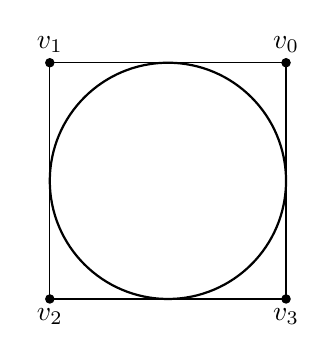
\begin{tikzpicture}[scale=1.5]
            \draw (1,1) -- (-1,1);
            \draw (1,1) -- (1,-1);
            \draw (-1,-1) -- (-1,1);
            \draw (-1,-1) -- (1,-1);

            \filldraw (1,1) circle (1pt) node[anchor=south]{$v_{0}$};
            \filldraw (-1,1) circle (1pt) node[anchor=south]{$v_{1}$};
            \filldraw (-1,-1) circle (1pt) node[anchor=north]{$v_{2}$};
            \filldraw (1,-1) circle (1pt) node[anchor=north]{$v_{3}$};

            \filldraw[color=black, fill=white, thick] (0,0) circle (1);
        \end{tikzpicture}
    \end{center}
    Probaremos que $\abs{K}\cong\s^{1}$. Denotamos por $\abs{\cdot}$ la norma euclideana y 
    $\norm{\cdot}$ a la norma que corresponde al máximo del valor absoluto de cada entrada. 
    Consideramos la función
    \begin{align*}
        f:\abs{K} &\to \s^{1}\htext{dada por} \\
        x &\to \frac{x}{\abs{x}}
    \end{align*}
    que resulta ser continua ya que $\abs{K}\subseteq\R^{2}\setminus\{0\}$. Afirmamos que 
    $g:\s^{1}\to\abs{K}$ dada por
    \begin{equation*}
        g(x):=\frac{x}{\norm{x}}
    \end{equation*}
    Notemos que $g$ esta bien definida, ya que $\{x\in\R^{2}\setminus\{0\}:\norm{x}=1\}=\abs{K}$. 
    Como $\norm{\cdot}$ y $\abs{\cdot}$ son normas equivalentes, inducen la misma topología y por
    lo tanto $g$ es continua ya que $\s^{1}\subseteq\R^{2}\setminus\{0\}$. Luego,
    \begin{equation*}
        f\circ g(x)=f\left(\frac{x}{\norm{x}}\right)
        =\frac{\frac{x}{\norm{x}}}{\abs{\frac{x}{\norm{x}}}}=x
    \end{equation*}
    es decir, $f\circ g=id_{\s^{1}}$. Del mismo modo, $g\circ f=id_{\abs{K}}$. Lo que prueba que
    $(K,f)$ es una triangulación de $\s^{1}$. Así, la característica de Euler de la triangulación
    es $V-E+F=4-4+0=0$.

    \item En $\R^{3}$ tomemos los puntos de la forma $(\pm1,\pm1,\pm1)$ que en total son $8$ y son
    vértices del cubo $[-1,1]^{3}$. Definimos el complejo simplicial $K$ que tiene por poliedro al
    cubo y que esta representado en la siguiente figura

    \begin{center} % Triangulación de la esfera
        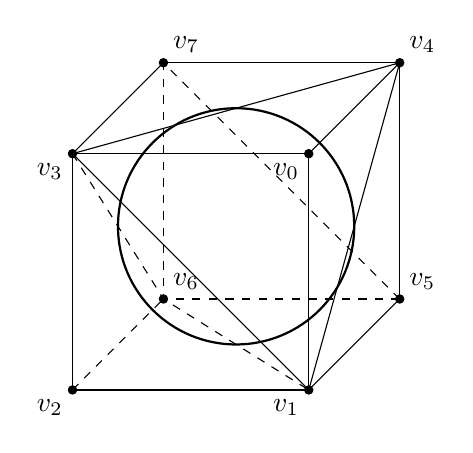
\begin{tikzpicture}[scale=1.5]
            \filldraw[color=black, fill=white, thick] (0,0,0) circle (1);
            
            \coordinate (A) at (1,1,1);
            \coordinate (B) at (1,-1,1);
            \coordinate (C) at (-1,-1,1);
            \coordinate (D) at (-1,1,1);

            \coordinate (E) at (1,1,-1);
            \coordinate (F) at (1,-1,-1);
            \coordinate (G) at (-1,-1,-1);
            \coordinate (H) at (-1,1,-1);

            \draw (A) -- (B) -- (C) -- (D) -- cycle;
            
            \draw (H) -- (E) -- (F);
            \draw[dashed] (F) -- (G) -- (H);

            \draw (A) -- (E);
            \draw (B) -- (F);
            \draw[dashed] (C) -- (G);
            \draw (D) -- (H);

            \draw (D) -- (E) -- (B);
            \draw (B) -- (D);

            \draw[dashed] (D) -- (G) -- (B);
            \draw[dashed] (F) -- (H);

            \filldraw (A) circle (1pt) node[anchor=north east]{$v_{0}$};
            \filldraw (B) circle (1pt) node[anchor=north east]{$v_{1}$};
            \filldraw (C) circle (1pt) node[anchor=north east]{$v_{2}$};
            \filldraw (D) circle (1pt) node[anchor=north east]{$v_{3}$};
            
            \filldraw (E) circle (1pt) node[anchor=south west]{$v_{4}$};
            \filldraw (F) circle (1pt) node[anchor=south west]{$v_{5}$};
            \filldraw (G) circle (1pt) node[anchor=south west]{$v_{6}$};
            \filldraw (H) circle (1pt) node[anchor=south west]{$v_{7}$};
        \end{tikzpicture}
    \end{center}
    Los puntos $v_{i}$ corresponden a los vértices del complejo, los segmentos a los $1-$simplejos 
    y también se consideran los $2-$simplejos encerrados por tres segmentos, por ejemplo, el 
    simplice $\sigma=\gen{v_{0},v_{3},v_{4}}$. Afirmamos que $\abs{K}\cong\s^{2}$. Del mismo modo 
    que antes definimos la función continua $f:\abs{K}\to\s^{2}$ dada por
    \begin{equation*}
        f(x)=\frac{x}{\abs{x}}
    \end{equation*}
    con inversa continua $g:\s^{2}\to\abs{K}$ dada por
    \begin{equation*}
        g(x):=\frac{x}{\norm{x}}
    \end{equation*}
    donde $\abs{\cdot}$ y $\norm{\cdot}$ son la norma euclideana y la norma del máximo 
    respectivamente. Concluimos que $(K,f)$ es una triangulación de $\s^{2}$ cuya característica
    de Euler es $V-E+F=8-18+12=2$.

    \item -
    
    \vspace{2mm}
    \noindent Triangulamos $[0,1]^{2}$ del siguiente modo,
    \begin{center} % Triangulación del cuadrado
        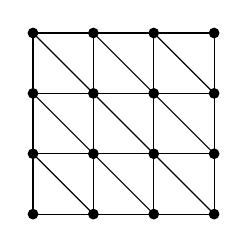
\begin{tikzpicture}[scale=2.3]
            \coordinate (A) at (0,0);
            \coordinate (B) at (1,0);
            \coordinate (C) at (1,1);
            \coordinate (D) at (0,1);
            
            \coordinate (E) at (1/3,0);
            \coordinate (F) at (2/3,0);
            
            \coordinate (G) at (1,1/3);
            \coordinate (H) at (1,2/3);

            \coordinate (I) at (2/3,1);
            \coordinate (J) at (1/3,1);

            \coordinate (K) at (0,2/3);
            \coordinate (L) at (0,1/3);

            \draw (A) -- (B) -- (C) -- (D) -- cycle;
            
            \draw (E) -- (J);
            \draw (F) -- (I);
            \draw (G) -- (L);
            \draw (H) -- (K);
            
            \draw (E) -- (L);
            \draw (F) -- (K);
            \draw (B) -- (D);
            \draw (H) -- (I);
            \draw (G) -- (J);

            \filldraw (A) circle (0.75pt);
            \filldraw (B) circle (0.75pt);
            \filldraw (C) circle (0.75pt);
            \filldraw (D) circle (0.75pt);

            \filldraw (K) circle (0.75pt);
            \filldraw (H) circle (0.75pt);
            
            \filldraw (L) circle (0.75pt);
            \filldraw (G) circle (0.75pt);

            \filldraw (E) circle (0.75pt);
            \filldraw (J) circle (0.75pt);
            \filldraw (1/3,2/3) circle (0.75pt);
            \filldraw (1/3,1/3) circle (0.75pt);

            \filldraw (F) circle (0.75pt);
            \filldraw (I) circle (0.75pt);
            \filldraw (2/3,2/3) circle (0.75pt);
            \filldraw (2/3,1/3) circle (0.75pt);
        \end{tikzpicture}
    \end{center}
    Donde cada vértice corresponde a un par ordenado con coordenadas en el conjunto 
    $\{0,1/3,2/3,1\}$, denotaremos por $V_{\square}$ al conjunto de vértices. Definimos 
    $f:V_{\square}\to V$ de modo que cada vértice en $V_{\square}$ se mapea a $\abs{K}$ como en la 
    siguiente figura,
    \begin{center} % Triangulación del cuadrado
        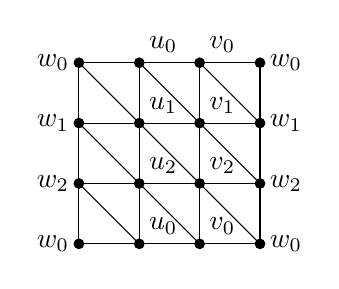
\begin{tikzpicture}[scale=2.3]
            \coordinate (A) at (0,0);
            \coordinate (B) at (1,0);
            \coordinate (C) at (1,1);
            \coordinate (D) at (0,1);
            
            \coordinate (E) at (1/3,0);
            \coordinate (F) at (2/3,0);
            
            \coordinate (G) at (1,1/3);
            \coordinate (H) at (1,2/3);

            \coordinate (I) at (2/3,1);
            \coordinate (J) at (1/3,1);

            \coordinate (K) at (0,2/3);
            \coordinate (L) at (0,1/3);

            \draw (A) -- (B) -- (C) -- (D) -- cycle;
            
            \draw (E) -- (J);
            \draw (F) -- (I);
            \draw (G) -- (L);
            \draw (H) -- (K);
            
            \draw (E) -- (L);
            \draw (F) -- (K);
            \draw (B) -- (D);
            \draw (H) -- (I);
            \draw (G) -- (J);

            \filldraw (A) circle (0.75pt) node[anchor=east]{$w_{0}$};
            \filldraw (B) circle (0.75pt) node[anchor=west]{$w_{0}$};
            \filldraw (C) circle (0.75pt) node[anchor=west]{$w_{0}$};
            \filldraw (D) circle (0.75pt) node[anchor=east]{$w_{0}$};

            \filldraw (K) circle (0.75pt) node[anchor=east]{$w_{1}$};
            \filldraw (H) circle (0.75pt) node[anchor=west]{$w_{1}$};
            
            \filldraw (L) circle (0.75pt) node[anchor=east]{$w_{2}$};
            \filldraw (G) circle (0.75pt) node[anchor=west]{$w_{2}$};

            \filldraw (E) circle (0.75pt) node[anchor=south west]{$u_{0}$};
            \filldraw (J) circle (0.75pt) node[anchor=south west]{$u_{0}$};
            \filldraw (1/3,2/3) circle (0.75pt) node[anchor=south west]{$u_{1}$};
            \filldraw (1/3,1/3) circle (0.75pt) node[anchor=south west]{$u_{2}$};

            \filldraw (F) circle (0.75pt) node[anchor=south west]{$v_{0}$};
            \filldraw (I) circle (0.75pt) node[anchor=south west]{$v_{0}$};
            \filldraw (2/3,2/3) circle (0.75pt) node[anchor=south west]{$v_{1}$};
            \filldraw (2/3,1/3) circle (0.75pt) node[anchor=south west]{$v_{2}$};
        \end{tikzpicture}
    \end{center}
    Luego, $f$ se extiende linealmente a una función continua continua de $[0,1]^{2}$ a $\abs{K}$.
    Como $f$ es sobreyectiva en vértices, se tiene que $f$ es cociente. Así, la función realiza 
    las siguientes acciones sobre $[0,1]^{2}$
    \begin{center} % Triangulación del cuadrado
        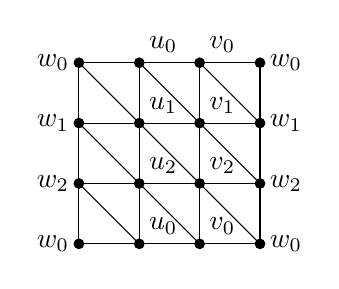
\begin{tikzpicture}[scale=2.3]
            \coordinate (A) at (0,0);
            \coordinate (B) at (1,0);
            \coordinate (C) at (1,1);
            \coordinate (D) at (0,1);
            
            \coordinate (E) at (1/3,0);
            \coordinate (F) at (2/3,0);
            
            \coordinate (G) at (1,1/3);
            \coordinate (H) at (1,2/3);

            \coordinate (I) at (2/3,1);
            \coordinate (J) at (1/3,1);

            \coordinate (K) at (0,2/3);
            \coordinate (L) at (0,1/3);

            \draw (A) -- (B) -- (C) -- (D) -- cycle;
            
            \draw (E) -- (J);
            \draw (F) -- (I);
            \draw (G) -- (L);
            \draw (H) -- (K);
            
            \draw (E) -- (L);
            \draw (F) -- (K);
            \draw (B) -- (D);
            \draw (H) -- (I);
            \draw (G) -- (J);

            \filldraw (A) circle (0.75pt) node[anchor=east]{$w_{0}$};
            \filldraw (B) circle (0.75pt) node[anchor=west]{$w_{0}$};
            \filldraw (C) circle (0.75pt) node[anchor=west]{$w_{0}$};
            \filldraw (D) circle (0.75pt) node[anchor=east]{$w_{0}$};

            \filldraw (K) circle (0.75pt) node[anchor=east]{$w_{1}$};
            \filldraw (H) circle (0.75pt) node[anchor=west]{$w_{1}$};
            
            \filldraw (L) circle (0.75pt) node[anchor=east]{$w_{2}$};
            \filldraw (G) circle (0.75pt) node[anchor=west]{$w_{2}$};

            \filldraw (E) circle (0.75pt) node[anchor=south west]{$u_{0}$};
            \filldraw (J) circle (0.75pt) node[anchor=south west]{$u_{0}$};
            \filldraw (1/3,2/3) circle (0.75pt) node[anchor=south west]{$u_{1}$};
            \filldraw (1/3,1/3) circle (0.75pt) node[anchor=south west]{$u_{2}$};

            \filldraw (F) circle (0.75pt) node[anchor=south west]{$v_{0}$};
            \filldraw (I) circle (0.75pt) node[anchor=south west]{$v_{0}$};
            \filldraw (2/3,2/3) circle (0.75pt) node[anchor=south west]{$v_{1}$};
            \filldraw (2/3,1/3) circle (0.75pt) node[anchor=south west]{$v_{2}$};
        \end{tikzpicture}
        $\to$
        % Paso intermedio de la triangulación del toro
        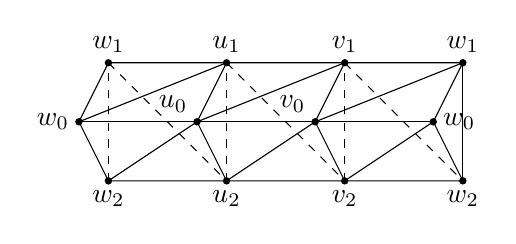
\begin{tikzpicture}[scale=1.5]
        \coordinate (A) at (0,0);
        \coordinate (B) at (0,1);
        \coordinate (C) at (-1/4,1/2);

        \coordinate (D) at (1,0);
        \coordinate (E) at (1,1);
        \coordinate (F) at (3/4,1/2);

        \coordinate (G) at (2,0);
        \coordinate (H) at (2,1);
        \coordinate (I) at (7/4,1/2);

        \coordinate (J) at (3,0);
        \coordinate (K) at (3,1);
        \coordinate (L) at (11/4,1/2);

        \draw (A) -- (J) -- (L) -- (K) -- (B) -- (C) -- cycle;
        \draw (J) -- (K);
        \draw (C) -- (L);

        \draw[dashed] (A) -- (B);

        \draw (D) -- (F) -- (E);
        \draw[dashed] (D) -- (E);

        \draw (G) -- (I) -- (H);
        \draw[dashed] (G) -- (H);

        \draw (C) -- (E);
        \draw (A) -- (F) -- (H);
        \draw (D) -- (I) -- (K);
        \draw (G) -- (L);

        \draw[dashed] (B) -- (D);
        \draw[dashed] (E) -- (G);
        \draw[dashed] (H) -- (J);

        \filldraw (A) circle (0.75pt) node[anchor=north]{$w_{2}$};
        \filldraw (B) circle (0.75pt) node[anchor=south]{$w_{1}$};
        \filldraw (C) circle (0.75pt) node[anchor=east]{$w_{0}$};

        \filldraw (J) circle (0.75pt) node[anchor=north]{$w_{2}$};
        \filldraw (K) circle (0.75pt) node[anchor=south]{$w_{1}$};
        \filldraw (L) circle (0.75pt) node[anchor=west]{$w_{0}$};

        \filldraw (D) circle (0.75pt) node[anchor=north]{$u_{2}$};
        \filldraw (E) circle (0.75pt) node[anchor=south]{$u_{1}$};
        \filldraw (F) circle (0.75pt) node[anchor=south east]{$u_{0}$};

        \filldraw (G) circle (0.75pt) node[anchor=north]{$v_{2}$};
        \filldraw (H) circle (0.75pt) node[anchor=south]{$v_{1}$};
        \filldraw (I) circle (0.75pt) node[anchor=south east]{$v_{0}$};
        \end{tikzpicture}
    \end{center}

    \vspace{2mm}
    \begin{center} % Triangulación del toro
        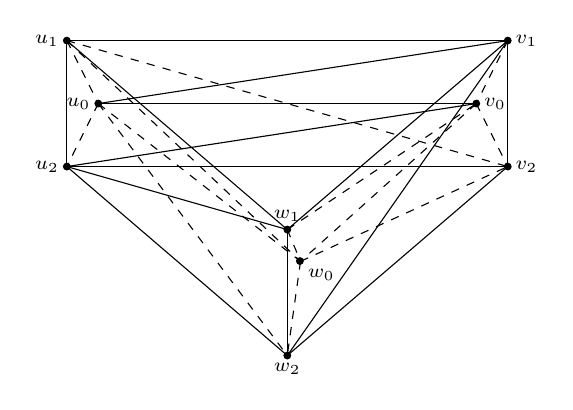
\begin{tikzpicture}[scale=0.8]
            \draw (-1.5,3.5) -- (5.5,3.5);
            \draw[dashed] (-1.5,3.5) -- (-1.,2.5);
            \draw[dashed] (-1.,2.5) -- (-1.5,1.5);
            \draw (-1.,2.5) -- (5.,2.5);
            \draw[dashed] (5.5,3.5) -- (5.,2.5);
            \draw[dashed] (5.,2.5) -- (5.5,1.5);
            \draw (-1.5,1.5) -- (5.5,1.5);
            \draw (-1.5,3.5) -- (-1.5,1.5);
            \draw (5.5,3.5) -- (5.5,1.5);
            \draw[dashed] (5.,2.5) -- (2.209699462447651,-0.004690804599365735);
            \draw[dashed] (-1.,2.5) -- (2.209699462447651,-0.004690804599365735);
            \draw (2.,0.5) -- (-1.5,3.5);
            \draw (-1.5,1.5) -- (2.,-1.5);
            \draw (2.,0.5) -- (5.5,3.5);
            \draw (2.,-1.5) -- (5.5,1.5);
            \draw[dashed] (2.,0.5) -- (2.209699462447651,-0.004690804599365735);
            \draw (2.,0.5) -- (2.,-1.5);
            \draw[dashed] (2.209699462447651,-0.004690804599365735) -- (2.,-1.5);
            \draw[dashed] (-1.5,3.5) -- (5.5,1.5);
            \draw (-1.,2.5) -- (5.5,3.5);
            \draw (-1.5,1.5) -- (5.,2.5);
            \draw (-1.5,1.5) -- (2.,0.5);
            \draw (2.,-1.5) -- (5.5,3.5);
            \draw[dashed] (2.209699462447651,-0.004690804599365735) -- (5.5,1.5);
            \draw[dashed] (2.,0.5) -- (5.,2.5);
            \draw[dashed] (-1.,2.5) -- (2.,-1.5);
            \draw[dashed] (-1.5,3.5) -- (2.209699462447651,-0.004690804599365735);

            \begin{scriptsize}
                \draw [fill=black] (2.,-1.5) circle (1.5pt) node[anchor=north]{$w_{2}$};
                \draw [fill=black] (2.,0.5) circle (1.5pt) node[anchor=south]{$w_{1}$};
                \draw [fill=black] (2.2,0) circle (1.5pt) node[anchor=north west]{$w_{0}$};
                \draw [fill=black] (5.5,3.5) circle (1.5pt) node[anchor=west]{$v_{1}$};
                \draw [fill=black] (5.5,1.5) circle (1.5pt) node[anchor=west]{$v_{2}$};
                \draw [fill=black] (5.,2.5) circle (1.5pt) node[anchor=west]{$v_{0}$};
                \draw [fill=black] (-1.5,3.5) circle (1.5pt) node[anchor=east]{$u_{1}$};
                \draw [fill=black] (-1.5,1.5) circle (1.5pt) node[anchor=east]{$u_{2}$};
                \draw [fill=black] (-1.,2.5) circle (1.5pt) node[anchor=east]{$u_{0}$};
            \end{scriptsize}
        \end{tikzpicture}
    \end{center}
    Sea $\pi$ la proyección a $\mathbb{T}^{2}$. Veamos que $f$ es constante en las fibras de 
    $\pi$ y viceversa. (...). Así, por propiedad universal de topología cociente, $f$ induce una 
    función continua $\rho:\abs{K}\to\mathbb{T}^{2}$ y del mismo modo $\pi$ induce una función 
    $h:\mathbb{T}^{2}\to\abs{K}$ también continua. Tenemos el siguiente diagrama,
    
    \vspace{2mm}
    \centerline{
        \xymatrix{
            [0,1]^{2} \ar[d]^{\pi} \ar[rd]^{f} \\
            \mathbb{T}^{2} \ar@{-->}[r]^{h} & \abs{K} \ar@{-->}@/^/[l]^{\rho}
        }
    }
    Veamos que $h$ es la inversa de $\rho$. Sabemos que $\rho\circ f=\pi$ y $h\circ\pi=f$. Luego,
    sea $y\in\abs{K}$, existe $x\in[0,1]^{2}$ tal que $y=f(x)$, así 
    $h\circ\rho(y)=h\circ\rho\circ f(x)=h\circ\pi(x)=f(x)=y$, por otro lado, 
    $\rho\circ h([x])=\rho\circ h\circ\pi(x)=\rho\circ f(x)=[x]$. Por lo tanto, $(K,\rho)$ es una 
    triangulación del toro. La característica de Euler es $V-E+F=9-$.
\end{enumerate}

%\printbibliography % Quitar el comentado si quiero usar bibliografia

\end{document}
